\documentclass[english]{scrartcl}
\pagenumbering{arabic}
\usepackage[utf8]{inputenc}
\usepackage[english]{babel}
\usepackage{amsmath}
\usepackage{amsfonts}
\usepackage{amssymb}
\usepackage{fancyvrb}
\usepackage{xspace}
\usepackage{refstyle}
\usepackage{hyperref}
\usepackage{listings}
\usepackage{enumitem}
\usepackage{graphicx}

% ============================================================
% Markup macros for proof-reading
\usepackage{ifthen}
\usepackage[normalem]{ulem} % for \sout
\usepackage{xcolor}
\newcommand{\ra}{$\rightarrow$}
\newboolean{showedits}
\setboolean{showedits}{true} % toggle to show or hide edits
%\setboolean{showedits}{false} % toggle to show or hide edits
\ifthenelse{\boolean{showedits}}
{
	\newcommand{\ugh}[1]{\textcolor{red}{\uwave{#1}}} % please rephrase
	\newcommand{\ins}[1]{\textcolor{blue}{\uline{#1}}} % please insert
	\newcommand{\del}[1]{\textcolor{red}{\sout{#1}}} % please delete
	\newcommand{\chg}[2]{\textcolor{red}{\sout{#1}}{\ra}\textcolor{blue}{\uline{#2}}} % please change
}{
	\newcommand{\ugh}[1]{#1} % please rephrase
	\newcommand{\ins}[1]{#1} % please insert
	\newcommand{\del}[1]{} % please delete
	\newcommand{\chg}[2]{#2}
}
% ============================================================
% Put edit comments in a really ugly standout display
%\usepackage{ifthen}
\usepackage{amssymb}
\newboolean{showcomments}
\setboolean{showcomments}{true}
%\setboolean{showcomments}{false}
\newcommand{\id}[1]{$-$Id: scgPaper.tex 32478 2010-04-29 09:11:32Z oscar $-$}
\newcommand{\yellowbox}[1]{\fcolorbox{gray}{yellow}{\bfseries\sffamily\scriptsize#1}}
\newcommand{\triangles}[1]{{\sf\small$\blacktriangleright$\textit{#1}$\blacktriangleleft$}}
\ifthenelse{\boolean{showcomments}}
%{\newcommand{\nb}[2]{{\yellowbox{#1}\triangles{#2}}}
{\newcommand{\nbc}[3]{
 {\colorbox{#3}{\bfseries\sffamily\scriptsize\textcolor{white}{#1}}}
 {\textcolor{#3}{\sf\small$\blacktriangleright$\textit{#2}$\blacktriangleleft$}}}
 \newcommand{\version}{\emph{\scriptsize\id}}}
{\newcommand{\nbc}[3]{}
 \renewcommand{\ugh}[1]{#1} % please rephrase
 \renewcommand{\ins}[1]{#1} % please insert
 \renewcommand{\del}[1]{} % please delete
 \renewcommand{\chg}[2]{#2} % please change
 \newcommand{\version}{}}
\newcommand{\nb}[2]{\nbc{#1}{#2}{orange}}
\newcommand{\here}{\yellowbox{$\Rightarrow$ CONTINUE HERE $\Leftarrow$}}

\newcommand\rev[2]{\nb{TODO (rev #1)}{#2}} % reviewer comments
\newcommand\fix[1]{\nb{FIX}{#1}}
\newcommand\todo[1]{\nb{TO DO}{#1}}
\newcommand\meta[1]{\nbc{META}{#1}{purple}}
\newcommand\jr[1]{\nbc{JR}{#1}{orange}}
\newcommand\nes[1]{\nbc{nes}{#1}{blue}}
\newcommand\on[1]{\nbc{ON}{#1}{red}} % add more author macros here
\newcommand\ewe[1]{\nbc{EWE}{#1}{olive}} % add more author

% ============================================================

\newcommand{\bs}{\symbol{'134}} % backslash
\newcommand{\us}{\symbol{'137}} % underscore
\newcommand{\ie}{\emph{i.e.}\xspace}
\newcommand{\eg}{\emph{e.g.}\xspace}
\newcommand{\etal}{\emph{et al.}\xspace}

\newcommand{\DD}{Dood\-le\-De\-bug\xspace}
\newcommand{\Doodle}{\texttt{Doo.\-dle}\xspace}
\newcommand{\println}{\texttt{Sys\-tem.\-out.\-println}\xspace}

% ============================================================

\begin{document}
\title{DoodleDebug}
\subtitle{A shot-gun marriage between System.out.println and object inspectors}
\maketitle

\begin{abstract}
Developers need effective ways to inspect and explore the run-time state of programs they are developing and debugging.  Modern debuggers and object inspectors are powerful tools, but they can only be used to explore specific points in the execution where breakpoints have been set. As a result, developers often resort to inserting ``print statements'' in code to log the state at multiple points in the execution. Print statements, however are a `poor man's debugger'', since their output is static and cannot be further explored.
We propose to combine the simplicity of print statements with the graphical sophistication and interaction of modern debugging tools.
\DD is a simple API modeled loosely after Java's \println. Objects that are ``printed'' generate graphical views that can be further explored, and can also be used to navigate back to source code in the IDE.
We introduce \DD and present the results of a usability study that shows that \DD can be very effective for common debugging tasks.
\end{abstract}

\section{Introduction}

For understanding and debugging a program, developers rely on tools to track its runtime states during execution.
One method is to insert print statements like \println in Java.
This method is quick and allows \del{its users}\meta{"allow" doesn't work without a dative} to compare different states in time of a specific object.
However, this output is static and comes with a couple of conceptual restrictions. On the one hand, the level of detail is hardcoded through the textual representations of objects.
If a developer decides for a simple and clear way of representation, they will need to rewrite their code for any further inspection and re-run the program after every change. \nes{That's be a problem in a long-running program.}
If they initially choose a detailed and verbose object representation, the output will grow and become tedious to read.
Another drawback of textual representation is caused by the simplicity of plain text.
It's one-dimensional and contains no information about graphical features like advanced formatting or colors. \nes{Obscure. Colors are a side-dish. What you want to advertise is *nesting*.}

The other half of the two most widely used debugging tools is the family of debuggers~\cite{Kras88a}.
When utilizing a debugger, a program can be stopped at a specific point of its execution, allowing developers to inspect any detail of this very state.
A clear advantage over textual output is the ability to inspect objects on demand.
Information is only displayed as soon as the user asks for it, nevertheless available without re-running the program.
The drawbacks of debuggers arise from the fact that their inspector is always bound to a specific point in time and therefore makes it impossible to directly compare different states of the same object.\nes{Nice.}

\DD combines the power of the above mentioned tools, erasing the conceptual problems coming with them.
Its output is is generated through an API taking its cue from \println's paradigms.
A developer simply needs to call \Doodle(object) to doodle any object type.
For simple customization of object representations, a class can implement the \texttt{Doodleable} interface which contains 2 methods, \texttt{doodleOn} and \texttt{summarizeOn}.
In contrast to Java's \texttt{toString}, there are two methods, allowing developers to create two levels of detail for representation.
This distinction \ugh{takes effect in the principle of Semantic Zoom} \cite{semantic-zoom}.
\ugh{Also, they do not generate plain text but draw content on a virtual canvas.}


\section{Existing Debugging Tools}
\nes{Move to the back, like it was in the paper. I'm a big fan of "related work" in the back of a paper.}
In the world of programming languages, there are two classes of widely used debugging tools:
Textual output like Java's \println and Debuggers.

\subsection{Textual Output}
Java's \println provides a default textual representation for any object, though only primitives and Strings render to a complete (and useful) output in terms of information. \nes{Unnecessarily vague. The rules are no longer than what you're writing: primitives look good; everything else, including arrays!, just gets classname+hashvalue}
\del{Default renderings are kept lean for other objects, but can be easily improved by overriding \texttt{toString}.}
Debugging by directly writing into source code may be easier and quicker than having to equip other debugging tools for a session\ref{some guy}.
Also, objects can be tracked over time, always \ugh{receiving a copy of it} a precisely defined points of execution.

\subsubsection{Best Practice For Textual Output}
For a detailed comprehension of how programmers use textual output for debugging, we wrote a script that searches for such methods in open source projects.
It analyzed SqueakSource, a hosting service for Smalltalk projects, searching for \texttt{printOn} methods, Smalltalk's equivalent to Java's \println.
\todo{Results}

\subsubsection{Missing Features On Textual Output}
Textual output is static.
As a consequence, users always face a trade-off between detail level and compactness.
If the output misses a bit of information, they will need to go back to the code, edit its rendering and re-run the whole program.

Formatting text-only output is restricted to the usage of text characters, tabs and line breaks. \nes{I think we had that nicer in the paper. Why's this a problem? Because it makes it hard to nest layouts. Evidence? We looked at a bunch of system.out.println, and so no nesting going on. This whole paragraph is a re-write of a paragraph in the paper. Maybe steal that one? You're an author after all …}
\ugh{Also, already printed text or line breaks cannot be reverted.
In particular, nesting complex objects in a consistent way is not possible in a trivial way without breaking the whole pattern of \println.}

\begin{figure}[h]
	\begin{lstlisting}
	an Array(
	MatrixTransform2x3(
		2.0 0.0 0.0
		0.0 2.0 0.0
	) MatrixTransform2x3(
		1 -0.707107 0.0
		0.707107 0.707107 0.0
	))
	\end{lstlisting}
	\caption{Textual visualization of an array of 2D-matrices, without DoodleDebug.}
	\figlabel{nested-matrix-problem}
\end{figure}

\subsection{Debuggers}
\nes{It's starting to feel very repetitive. DD is positioned between println and Debuggers - fine. Why does that need so many headings and paragraphs?
There's no need to repeat the introduction.}
Debuggers allow users to stop a program's execution at any line of source code.
When stopped, any detail of the current state is inspectable.
Unlike \println, debuggers allow their users to put additional or remove existing break points at runtime, which makes changing the target piece of code to debug quicker, especially because the current program state doesn't need to be re-created like on a new run.

\subsubsection{Drawbacks Of Using A Debugger}
Since a debugger only shows the program's state at one point in time, comparison of two time slices is hardly possible.
Important details may only be memorized and mentally compared to the ones at a later point in time.

Eclipse's built-in Java debugger brings no options to customize its output.
When inspecting an object, all its fields are listed by name, coming along with a textual representation.
An object with many for a programmer unimportant fields may suffer the loss of its clarity from that.


\section{Features}
\meta{Completely rearranged this section. Smart implementation examples are now nested in "Configuration-free". Also, subsections are ordered by importance (my opinion).}
\todo{introduction text}

\subsection{Lean API}
The \DD API is lean.
It features three ends for developers to interact with it, though most will only ever use the first two.
\begin{itemize}
\item The \texttt{Doo.dle(Object)} method as a drop-in replacement for \println
\item The \texttt{Doodleable} interface and the associated interface \texttt{DoodleCanvas}, in which objects can define simple custom representations
\item The \texttt{RenderingPlugin} interface, which allows developers to provide powerful custom renderings for any type, based on HTML and CSS; source code access is not required here.
\end{itemize}
Altogether, \DD features no more than 10 public methods.

\subsection{Configuration-Free}
A key question in the design of a user interface is the level of configurability exposed to users.
Highly customizable solutions may be better for power users that are very familiar to the software in question.
Other users may always remain on default settings, independent of their fittingness.
We followed the advice of Norman\cite{?} and Buxton\cite{?}, which says not to treat everyone as a designer, but rather take away design decisions from users by creating sophisticated defaults.
As a consequence, there is no settings dialogue or file for \DD.

\subsubsection{Smart Scrolling}
In general, an output console can either move its view port to the bottom when new content is appended or stay where it was before.
\DD implements the scrolling behavior of MUSHClient\footnote{\url{http://www.gammon.com.au/mushclient/}} and mIRC\footnote{\url{http://www.mirc.com}}:
The view port will only be moved to the bottom if it already was before new content was added.
If the user doesn't scroll away from the bottom, they will benefit from notifications about new doodles.
On the other hand, users can scroll up to an old doodle without being bounced away when new objects are doodled.

\subsubsection{Notifications}
\seclabel{smart-focus}
When new objects are doodled, \DD autonomously decides whether to set focus to the \DD output view for user notification or not.
The crucial factor for this decision is the elapsed time since the last doodling.
Focus is gained if more than 4 seconds have passed and always for the first doodle of a program run.

When debugging a program with many output events per second, like a game, there is no sense in always notifying the user.
Either they keep their attention on the output as they see it's rapidly changing, or they work somewhere else in the UI and don't want to be pulled back every time.

Users that debug a program that rarely produces output, like caught exceptions, they probably want to be notified about this event and maybe inspect the new doodle. \nes{Connect with the study.}


\subsection{Inspection of Doodled Objects}
To avoid the trade-off between detail level and compactness, we implemented the principle of \emph{semantic zoom} along with \DD:
Every object features two levels of detail for its rendering.
Objects that are nested into others are not graphically scaled down nor removed, but rendered in its summarized, less detailed  version.

In \DD, objects rendered to nesting levels 0 (doodled ones) and 1 are rendered with full detail; objects of nesting level 2 (inside level 1) show their summarized version.
Clicking on a level 1 object opens a popup window only showing this very object, but with more detail since it's on the new nesting level 0 now.
Level 1 object in this window can again be clicked in order to inspect those.
This can be repeated until any leaf of the object tree is reached.
\Figref{addressbook_whole} shows a doodled address book (on level 0) containing several contacts (on level 1). Clicking on one of them creates a pop-up window, moving the respective contact object to new level 0 (\Figref{addressbook_contact}).

Navigation between nesting layers inside a pop-up is aided with bread crumbs~\cite{Krug00a} \nes{Page?}, which traces the currently inspected branch of the object graph (\figref{breadcrumbs}).
Any parent doodle in this trace can be clicked to jump to it directly.
When zooming out of the graph this way, the just visited branch is still visible in the breadcrumbs area until the user turns into a new path.

\begin{figure}[h]
	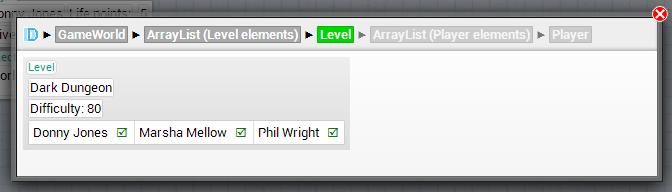
\includegraphics[width=\linewidth]{img/breadcrumbs.png}
	\caption{The labels at the top are \emph{bread crumbs}. The developer is currently looking at a \texttt{Level} object, which is the member of an ArrayList, which is the member of a \texttt{GameWorld}. The object that was doodled was the \texttt{GameWorld} object. The developer was previously zoomed in to player but zoomed out again to Level.}
	\figlabel{breadcrumbs}
\end{figure}

\subsubsection{Tracking an Object Over Time}

Thanks to \DD's inspection feature, the summarized representation of an object can be held rather terse.
As an example, the state of a game can be doodled on every update cycle like in \figref{game_long-list}.
A developer observing this output might be interested in more detail of one particular state, which can be done by clicking on parts of it, resulting in a pop-up (\figref{game_last-state}).

The program code defining a \texttt{Player}'s rendering looks as follows:
\begin{lstlisting}
public class Player implements Doodleable {
	public void doodleOn(DoodleCanvas c) {
		c.draw(name);
		c.newLine();
		c.draw("Alive?");
		c.draw(isAlive);
		c.newColumn();
		c.draw("Life points:");
		c.draw(lifePoints);
	}

	public void summarizeOn(DoodleCanvas c) {
		c.draw(name);
		c.draw(isAlive);
	}
}
\end{lstlisting}

\begin{figure}[h]
	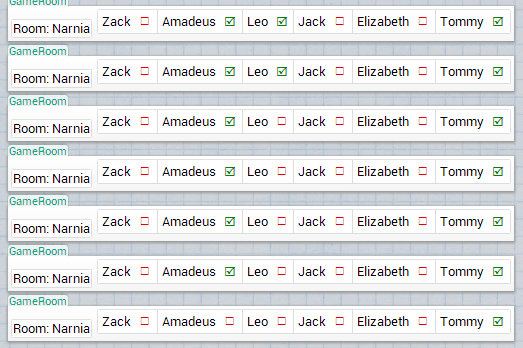
\includegraphics[width=\linewidth]{img/game_long-list.png}
	\caption[Example of a chronological sequence: Game]{A DoodleDebug console showing the doodles of \texttt{GameRoom}s. The boxes beside each are summarized booleans and indicate if the player is alive.}
	\figlabel{game_long-list}
\end{figure}

\begin{figure}[h]
	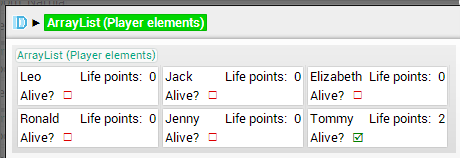
\includegraphics[width=\linewidth]{img/game_last-state.png}
	\caption[Example of a chronological sequence: Detailed player list]{Details of a \texttt{GameRoom} from \Figref{game_long-list}.}
	\figlabel{game_last-state}
\end{figure}

\begin{figure}[h]
	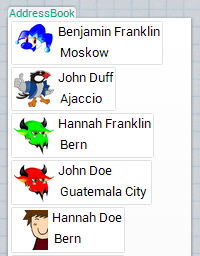
\includegraphics{img/AddressBook_whole.png}
	\caption[AddressBook visualization]{An address book only showing the summaries of its addresses. Clicking reveals the details in \Figref{addressbook_contact}.}
	\figlabel{addressbook_whole}
\end{figure}

\begin{figure}[h]
	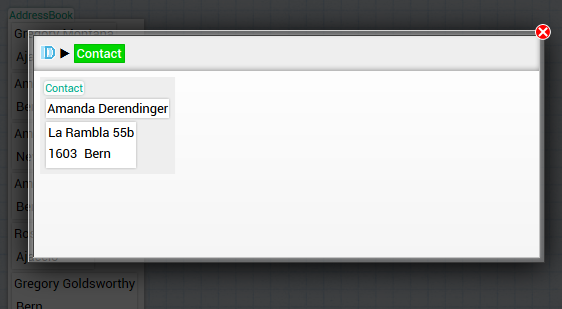
\includegraphics{img/AddressBook_contact.png}
	\caption[Contact visualization]{A popup showing the details of an address.}
	\figlabel{addressbook_contact}
\end{figure}

\subsection{Built-in Renderings}
\DD comes with predefined renderings for a number of commonly used data types in Java.
Those include:
\begin{itemize}[noitemsep]
\item Primitives
\item Arrays
\item Booleans
\item Classes
\item Collections
\item Colors
\item Images (various types)
\item Maps
\item Nulls
\item Objects (default)
\item Strings
\item Tables (rectangular two-dimensional arrays and collections)
\item Trowables
\end{itemize}


\subsection{Customization API}
\DD's API features two API layers for customization.
One layer, the Doodleable interface, utilizes a similar paradigm as Java's \texttt{toString()} method and targets most use cases since it's a simple and quick solution.
For more power and flexibility, users may also provide \texttt{RenderingPlugin}s, which are also used internally for \DD's built-in renderings.
However, \texttt{Doodleable} customizations are always preferred over plugins when both are available for a type.

\subsubsection{The Doodleable Interface}

The \texttt{Doodleable} interface features two methods: \texttt{doodleOn(DoodleCanvas)} for a regular representation and \texttt{summarizeOn(DoodleCanvas)} for a simplified and compact version.
Distinguishing between them enables semantic zoom \cite{semantic-zoom} when inspecting doodles.

\paragraph{DoodleCanvas}
Instead of creating a string like in \println, both methods receive a \texttt{DoodleCanvas} object for drawing contents on it.
The paradigm behind \texttt{DoodleCanvas} adopts the formatting of text in terms of lines and columns.
A virtual cursor starts at the upper-left corner of the canvas.
Drawn objects align one beside each other until a new line is created, which causes the cursor to jump back to the left which one line height offset.
The second formatting option is to create new columns, moving the cursor to a position on top, to the right of the right-most previous object.
\texttt{DoodleCanvas} therefore has three public methods: \texttt{draw(Object)}, \texttt{newLine()} and \texttt{newColumn()}.
\Figref{canvas-illustration} shows an example of how the \texttt{Doodleable} interface could be used on a \texttt{Contact} object.

\begin{figure}[h]
	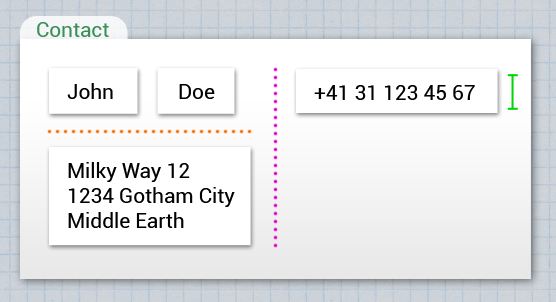
\includegraphics[width=\linewidth]{img/doodleable-example.png}
	\caption[Usage of the \texttt{Doodleable} interface]{Example of a \texttt{Contact} class' \texttt{doodleOn()} method.
Dotted lines visualize the effect of the structuring methods \texttt{newLine()} (orange) and \texttt{newColumn()} (purple).
The green i-beam indicates the final position of the canvas' imaginary cursor.}
	\figlabel{canvas-illustration}
\end{figure}

\subsubsection{Plugins}
There are cases where implementing the \texttt{Doodleable} canvas is not a satisfying option for developers.
If they don't have access to the source code, there is no (clean) way to add an interface.
Also, the \texttt{Doodleable} API only provides rough formatting options.

\paragraph{Implementing Plugins}
For advanced arrangement or additional features like coloring, \DD includes the option to provide plugins.
They must implement \texttt{RenderingPlugin}, which is most easily done by extending the built-in \texttt{AbstractPlugin}.
Each plugin holds information about the object types it is able to render.
Instead of drawing to a virtual canvas, a plugin receives a html \texttt{Tag} object and renders its own HTML code into this tag.
The principle of semantic zoom is again retained through two different methods for different detail levels.
In addition to HTML code generation, plugins have the option to cleanly provide CSS rules and individually adjust class attributes assigned to object doodles.


\section{Design}
For the design of \DD's output, we consulted literature to carefully plan the different project cycles.
As suggested by Buxton\cite{?}\todo{citation}, we decided to start with an initial design phase, which later fades into implementation as soon as a reasonable concept is available.
In particular, we started off by sketching parts of the future user interface with pen and paper and confronted possible users with them.
They were not told what a specific picture would represent, but directly had to state their intuition of what they believed it to be (\figref{sketch-discussion}).
Based on their feedback, we had an estimation of every sketch's quality in terms of intelligibility and could either keep, improve or dismiss it.
This cycle was repeated until our sketches reached a form where they were easily understood by people and we could start implementing.

Since the pen and paper sketches were rough and drafted quickly, the implementation phase initially revealed minor usability problems that had not been obvious in the design phase.
Those were vanished dynamically, still following Buxtons idea of gradually reducing design while implementation slowly starts.

\begin{figure}[h]
	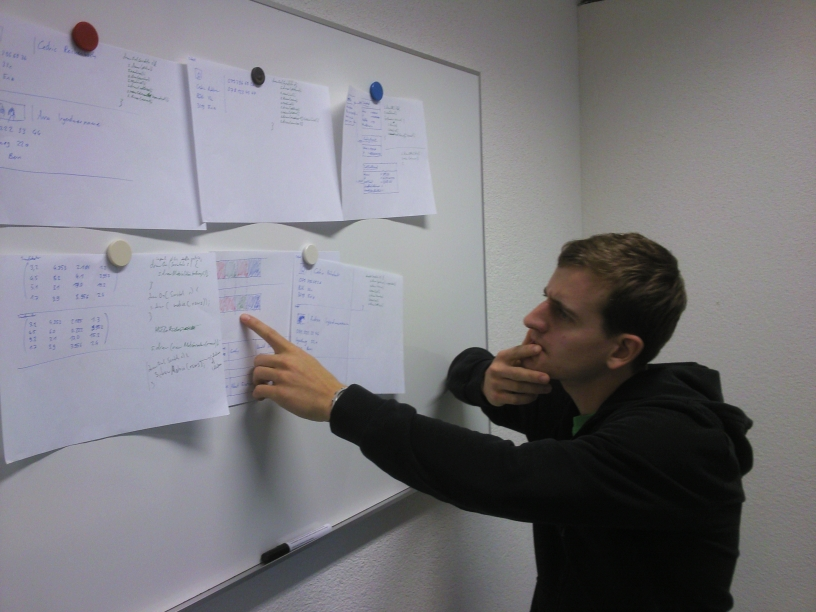
\includegraphics[width=\linewidth]{img/design-sketches_thinker.jpg}
	\caption[Confronting people with design sketches]{Programmer reacting to our sketches.}
	\figlabel{sketch-discussion}
\end{figure}

\begin{figure}[h]
	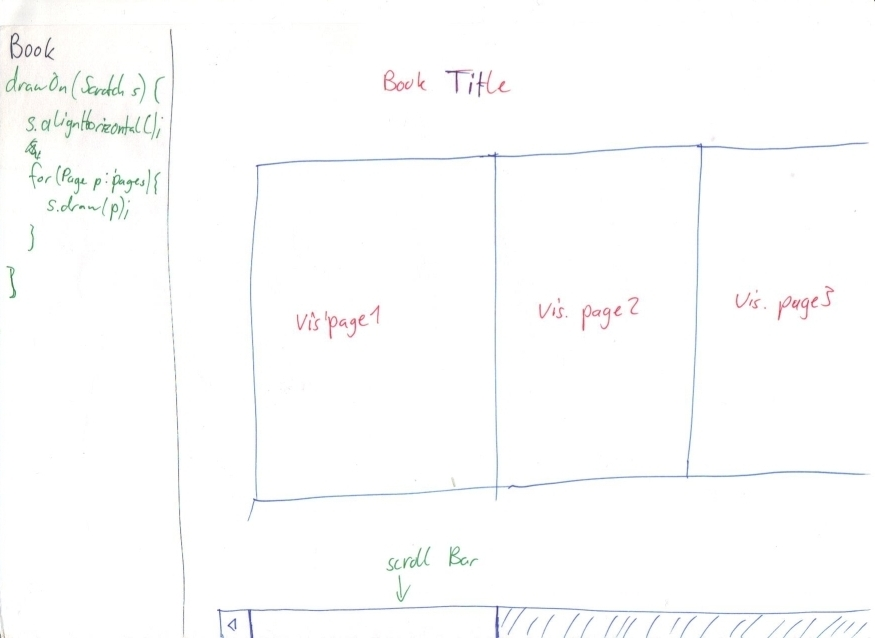
\includegraphics[width=\linewidth]{img/sketches/032.jpg}
	\caption[Bad sketch example: Horizontal and vertical alignment]{Inspired by Swing's FlowLayout, all objects are aligned horizontally.}
	\figlabel{bad-sketch_align-h-v}
\end{figure}

\begin{figure}[h]
	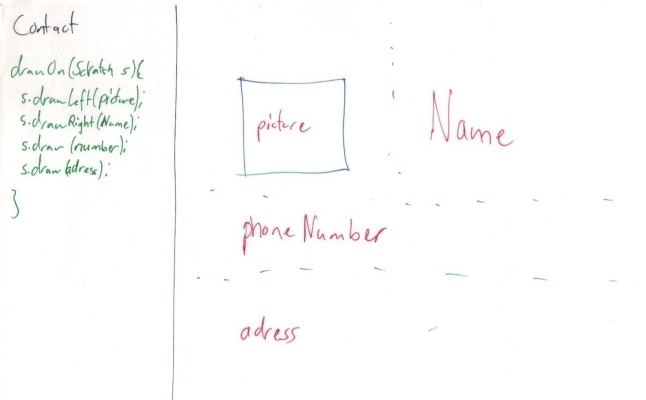
\includegraphics[width=\linewidth]{img/sketches/026.jpg}
	\caption[Bad sketch example: Left-right pattern]{A proposed canvas API that traverses the canvas from top to bottom, dividing it into virtual lines.}
	\figlabel{bad-sketch_left-right}
\end{figure}


\section{Implementation}
This section outlines the architecture and mechanisms \DD uses in order to perceive data, process them and display the results.

\subsection{Data Transport}
Since \DD is an Eclipse plugin, it's always running in a different Java VM than the project to be debugged itself.
As a consequence, object data needs to be transported after each \Doodle call.
\DD uses a third-party library\cite{xstream} to serialize doodled objects to XML, then transports the result as string over a connection on localhost using SIMON\cite{simon}.

\subsection{Rendering}
After a request for doodling an object has been received, \DD analyzes its type and searches for a fitting rendering in the different customization layers.
If none is available, a default rendering is used.

\subsubsection{Traversing Object Types}
Renderings are iteratively searched for all types and supertypes of an object, starting at the innermost type, defined through the object's class name.
As long as no rendering has been found, the algorithm traverses the inheritance tree in a layer-wise manner, always preferring the class type over interface types inside a layer.
In other words, this algorithm starts searching on the object's direct class and interface types, then goes on for the class' and interface's direct ancestors and repeats until a match was found or all leaves were reached.
The only type excluded from this search is the \texttt{Object} type, since it might be reached before some interface types.

\subsubsection{Output}
As output format, we decided to use HTML.
This enables great formatting possibilities with moderate implementation effort.
Eclipse provides the package \texttt{org.eclipse.swt.browser}, which includes a browser that easily blends into the Eclipse UI.
\nes{Previous sentence is advertisement. Rewrite.}
The rendering used for this browser's content is always the one from the OS's built-in browser and cannot be changed.
On Windows systems, for instace\nes{instance.}, Eclipse uses the Internet Explorer rendering engine.
\nes{Maybe spend a second or two talking about compatibility modes.}
As a consequence, we had to be careful when creating HTML output and always test them in different browsers to prevent differences in design on different systems.
\nes{More detail.}

\section{User Study}

\seclabel{study}
We carried out a usability study \cite{Krug00a} to validate the design of \DD.
Usability studies are qualitative rather than quantitative, offering deeper semantic insights~\cite[pp. 13--15]{Lang09b} than a quantitative study while simultaneously being easier to set up.
We pose three different problems to each test subject to be alternately solved with or without DoodleDebug, recording with screen capture videos and think aloud protocol.~\cite{Krug00a,Lang09b}
We search for problematic situations experienced with one tool and see if they've been solved more easily using other tools.
Seven developers solved 3 tasks each.

\subsection{Study Session Setup}
A fully functional release candidate of DoodleDebug was used.
\nes{Build number}
\meta{Well, I didn't really have a structured versioning before 1.0. Also, those are not publicly available (unless we move the whole git repo to github or whatever).}
It ran inside Eclipse 4.2 (Classic edition), using a ThinkPad T410 with Windows 7 (x64) and an external mouse.
The screen was captured during the whole session and one instructor sitting beside the test subject for problem explanation and protocol.
Before the actual testing, the user had 15--30 minutes to work through a tutorial and play around with DoodleDebug inside a sandbox.
At this time, the instructor was allowed to answer questions and support the subject.
\nes{Both, DD and debuggger?}
\meta{When going through the tutorial, you don't use the debugger. No one did. Or what do you mean?}

For the actual session, there were 3 different small programs containing some manually inserted bug, which they had to find and eliminate. 
For one or two of them, they were allowed to use DoodleDebug and for the other one or two respectively, they had to fall back to classical tools. 
The permission to use DoodleDebug on a particular problem changed with every study session, i.e.  if subject 1 was allowed to use DoodleDebug on problem A, then subject 2 would not be allowed, but subject 3 would. 
The reason for letting some subjects only use classical debugging tools was to have a reference of behavior in order to show that they are not trivial and detect what particular sub-problems they pose in detail, so we would see if DoodleDebug enables better approaches to solve them. 

Subjects worked on a problem until it was completely solved, none of them needing more than 30 minutes for any particular problem.

\nes{One thing we should mention, both here and in the paper, is that while some problems might not be especially fair, they nonetheless show that DD has strong points.}
\subsection{Posed Problems}
In the first two tasks, the participants are given a failing unit-like test. They are informed that the test is correct, and asked to fix the bug and thus have the test pass. Subjects have access to all of the source code and are allowed to manipulate it.

The selection of tasks intends to expose problem situations where \DD is superior to classical debugging tools rather than trying to cover most common debugging cases.

\subsubsection{Sorting}
A couple of gray scale \texttt{Color} objects are put into a \texttt{List} 
and then sorted using a custom \texttt{ColorComparator}, which should sort by brightness. 
The result then is compared in a unit test to a hand-built \texttt{List} which initially has the expected order.\\
Solution: In the comparator, completely black colors are wrongly treated as complete white.

\subsubsection{Serialization}
Phone book contacts are modeled using \texttt{Con\-tact} and \texttt{Address}  objects. 
They should be serialized using a \texttt{Ser\-ializ\-ing\-Util} (simulated serialization only) and de-serialized afterwards.
In a unit test, comparison of a contact object before and after serialization fails.\\
Solution: In the \texttt{SerializingUtil}, every field of type \texttt{long} is cast % NB: not "casted"
into an \texttt{integer} before serialization and back into a \texttt{long} afterwards. 
This causes a field called \texttt{phoneNumber} of \texttt{Address} to be changed into some negative value.

\subsubsection{Decimal Alignment}
In the third and last task, a class \texttt{DatabaseUtil} is given without source code, as a black box simulating access to an imaginary database by returning a two-dimensional array of \texttt{float}s when calling its only method \texttt{getData()}. 
Subjects are informed that in the returned table there are duplicated tuples and have to name them.

\subsection{Subjects}
\nes{Move this up.}
The subjects were convenience-sampled and assured of their anonymity. We informed them about the purpose of our study beforehand, and neither promised nor gave any reward for participating. The participants are enumerated in order of their participation.

\begin{description}
% Oskar Truffer
\item [{Alpha}] B.Sc in Mathematics, Minor in computer science. Now master student in computer science. % 60 ECTS
% Remo Diethelm
\item [{Bravo}] B.Sc. in Computer Science. Master Student  in Computer Science.
% Andrei Chis
\item [{Charlie}] M.Sc. in Computer Science. Ph.D. Student in Computer Science.
% Julian Schelker
\item [{Delta}] B.Sc. in Computer Science. Master Student  in Computer Science.
% Raffael Krebs
\item [{Echo}] M.Sc. in Computer Science. B.Sc. Working as Software Engineer, 1 year of industry experience. Experience in Eclipse plugin development
% Roger Kohler
\item [{Foxtrot}] B.Sc. in Computer Science. Master Student  in Computer Science.
% Ueli Scheidegger
\item [{Golf}] Lic.rer.pol. in Economics, Minor Computer Science. Working as Software Engineer, 15 years of industry experience. % 60 ECTS
\end{description}

\subsection{Observed behavior}
For four study subjects, \texttt{toString()} was used as the default rendering.
Two of them, Bravo and Delta, were allowed to use DoodleDebug for solving the serialization problem and both implemented \texttt{Doodleable} with \texttt{Contact} and \texttt{Address}.
For three subjects, the ObjectDoodler (which shows all instance variables) was the standard rendering.

\begin{tabular}{l | c c c}
 & \textbf{Sorting} & \textbf{Serialization} & \textbf{Table} \\
\hline
Alpha & DD & Classic & - \\
Bravo & Classic & DD & - \\
Charlie & DD & Classic & DD \\
Delta & Classic & DD & Classic \\
Echo & DD & Classic & DD \\
Foxtrot & Classic & DD & Classic \\
Golf & DD & Classic & DD \\
\end{tabular}

\subsubsection{Observations using System.out.println}
5 out of 7 subjects (all except Delta and Echo) made use of this mechanism to visualize runtime data. 
Alpha argued with laziness to open a debugger or to stare at foreign code. 
When quizzed, alpha said they can compare things, either two different objects as posed in the sorting problem or the same object at different points in time, as in the Serialization problem. 
Both are not directly possible with a classical debugger like the one built into Eclipse classic.

\paragraph{Homogenous Output}
Ad-hoc textual prints of the subjects were unstructured for all subjects except Charlie \meta{His structure is mentioned in the next paragraph, should we refer to that?}.
Beta printed each element of the wrongly sorted color list and then stared at the (unaligned) numerical values of red, green and blue color components. 
Once he found out that a black element was at the end instead of the beginning, he went on to investigate the cause, leading to the problem.

In contrast, subjects using DoodleDebug already had built-in renderings for \texttt{Collection}  and \texttt{Color}, making the problem immediately obvious.

\paragraph{Uninspectable and Useless Output}
The standard implementation of \println prints only the class name and object hash. 
Bravo and Golf resorted to a compile-run cycle, where they would explore the object graph by re-running the program, adapting the print statement to explore the parts of the object graph they were interested in.

Charlie was the only subject to override \texttt{toString()} methods, after being dissatisfied with the standard printout of class name plus hash. He implemented \texttt{toString()}  to print out all fields of an object, as seen in \Figref{charlie}. 

Alpha produced a very similar output, but instead of overriding \texttt{toString()}, he extracted all fields from outside using getter methods directly inside the \println method. 

\begin{figure}[h]
\begin{lstlisting}
public class Contact { ...
  public String toString() {
	return "name: " + name
		+ ", address: " + address;
  }
}
public class Address { ...
  public String toString() {
	return "street: " + street
	  + ", phoneNumber: " + phoneNumber
	  + ", city: " + city;
  }
}
\end{lstlisting}
  \caption{Participant overwrote \texttt{toString()} to aid debugging.}
  \figlabel{charlie}
\end{figure}

Another approach to solve insufficient output was to switch from \println to the debugger, observed with Bravo and Foxtrot.

\subsubsection{Observations using a Debugger}
Four subjects (Bravo, Delta, Echo and Foxtrot) used the Eclipse debugger to inspect objects, only Delta and Echo using it exclusively. 
Echo's argumentation for this usage was that debuggers are more powerful in comparison to \println, because they allow one to inspect objects dynamically and additionally provide simple improvements of standard textual representations (\eg arrays are represented in the form of \texttt{[objectA, objectB, ...]}instead of \texttt{[Ljava.lang.Object;@4cb162d5}.
Echo mentioned that they missed the feature to compare two objects from different points in time.

\paragraph{Comparison Between Objects}
The built-in Eclipse debugger only allows you to inspect one object at one point in time. 
As the serialization problem consists of two objects unexpectedly  being unequal, part of the debugging process was somehow comparing them in order to find their difference. 
Every subject except Golf did this --- Golf only tried to understand the serialization and de-serialization process to find out where the implementation has mistakes. 
Echo never used \println, but attempted to compare objects before and after serialization using the debugger. 
Even though the debugger supported simple and fast inspection to any point inside the object, Echo explicitly pointed out that he missed the feature to inspect two objects simultaneously instead of memorizing small pieces and going to the other one for comparison.

\paragraph{Non-Selective Output}
Eclipse's Java debugger simply lists all contents of an object, since there is no information about relevance of its respective parts. 
In particular, interfaces may specify an imaginary concept and be used in the declaration context for better overview, but for creation of an instance, a full class implementing this interface is needed. 
The debugger is working at runtime and therefore only knows the instantiated type of an object, so it will visualize all properties and contents of this, potentially resulting in a overly verbose output. 
We observed this on the color list problem, where \texttt{ArrayList} 
was used as implementation for the interface \texttt{List}.
Subject Bravo initially tried to perceive the structure of a list right after sorting by pausing the program  using the debugger and inspecting the mentioned list (\Figref{debugger_color-list}), but instantly gave up and switched to writing a \texttt{for} loop which sequentially prints out all elements using \println. 
\todo{Screenshot of \texttt{Doodleable} usage}
\begin{figure}[h]
	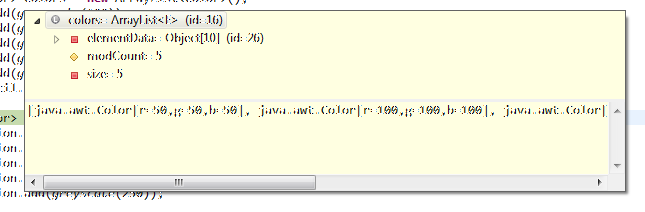
\includegraphics[width=\linewidth]{img/debugger_color-list_remo.png}
	\caption[Bravo using the debugger for a color list]{Eclipse's debugger visualizes all fields of an object's runtime type (ArrayList)}
	\figlabel{debugger_color-list}
\end{figure}

\subsubsection{Observations using DoodleDebug}
\todo{adjust introduction (was copied from somewhere else}
Foxtrot was the only one to use DoodleDebug on the serialization problem \meta{Nope... Why did I write this?}.
He simply doodled the problematic \texttt{Contact} object before and after serialization.
Based on the \texttt{ObjectPlugin}'s rendering, he found the problem (a changed phone number in address) in a matter of seconds.

\paragraph{Two methods in \texttt{Doodleable} interface}
Echo bespoke confusion about the difference between the two methods in the \texttt{Doodleable} interface. After going back to the documentation of the interface, he understood.
Alpha did not show any reaction when implementing the \texttt{Doodleable} interface for the first time, but simply delegated the zoom mechanism by replacing \texttt{c.draw(object)}from their \texttt{doodleOn.(Canvas)} 
by \texttt{c.drawSmall(object)} in their \texttt{summarizeOn.(Canvas)}.

\paragraph{Console Keeps Stealing Focus}
\seclabel{console-focus-problem}
When certain output is printed onto the console, it gains the UI's focus by default.
Due to the problem setup, every program initially threw an exception at the end of its execution, signaling the problem had not been solved yet.
Every user experienced the following problem at least once: They were using DoodleDebug and therefore had this view tab opened when the exception was thrown and Eclipse switched to the console.
Only Echo managed to disable its focus-on-change setting, while the other subjects just switched back to the DoodleDebug view tab after a few seconds.

\paragraph{Problem immediately obvious}
Charlie doodled both the wrongly sorted color list and the correctly sorted one. Since they were both on-screen immediately, he instantly noticed both their similarity and the difference, which was that the black color was on the wrong side of one list.

On the serialization problem, all three subjects (Bravo, Delta, Foxtrot) using DoodleDebug managed to find the changed field instantly after calling \texttt{Doo.dle()} once before and once after the de-/serialization step. That's because DoodleDebug's \texttt{ObjectPlugin} shows all instance variables, which was enough to immediately see the problem.

\paragraph{Default doodles were useless}
If the standard output of DoodleDebug does not fit a users needs, it can be adjusted through one of the two described methods; the simpler \texttt{Doodleable} interface was used in this context by Alpha while solving the sorting problem.
They included all instance variables of the questioned object for its representation.
On other sessions, Golf iteratively re-ran the program, each time printing another field of the same object and Bravo wrote a custom textual representation, printing all fields labelled with their names.

Based on this finding, we modified DoodleDebug's standard rendering: Instead of falling back to the object's \texttt{toString()} method, its fields are listed, containing field name and field content as a clickable sub-doodle in \Figref{fielddoodler-player}.

\subsubsection{Observations Without Any Debugging Tool}
Subject Gold was the only one to solve a problem without using any debugging tool.
On the serialization problem, they tried to comprehend the logic of the problem's \texttt{SerializingUtil}.
Unlike others, they found the problem source at the same time as the nature of the problem itself.
They fixed the bug and verified the result using \println.

\subsection{Summary}
Our study showed that \DD is clearly superior to both, \println and debuggers in certain debugging situations.
\DD addresses several issues of other tools and successfully vanishes them.
However, no conclusion can be drawn about its improvement for overall programming work due to the study's small size and its qualitative nature.

\section{Future Work}
There are a couple of ideas that might enhance debugging experience and efficiency.
However, they'd need to be tested to verify their usefulness, possibly before implementing them.

\subsection{Highlighting Object Diffs}
When tracking and object over time, the most important information is located where properties of an object have changed.
Therefore, a mechanism comparing objects when they are doodled multiple times could be a powerful feature.

\subsection{Clickable Doodles}
One problem of using \println over a long period of time is, that it's indeed clear which object is printed, but not where the \println class has been made.
To find it, some tedious text search over the whole project is needed in the worst case.
As a solution in \DD, doodles could include a link pointing to the line in source code where the \Doodle call was triggered, similar to the way Throwables are tracked.

\subsection{Debugger Integration}
Since the eclipse debugger only uses textual representations and doesn't allow any customization, a way to enhance it could be to include doodles.
A user would be allowed to switch from the standard textual mode to \DD mode, where an object would be inspected using \DD's rendering.
Or a button beside the textual representation would create a popup with the doodled version of it.

\section{Conclusion}
\meta{Was a bit lost in this section, didn't really know what to write.}

\DD is a valuable drop-in replacement for Java's \println.
It introduces techniques to enhance debugging output by adopting well-proven mechanisms from debuggers and console printing on the one hand and introducing simple new ones on the other hand.
Getting started is rather easy since the setup work is mainly done by Eclipse and the API is simple; knowing one single method already enables the core features of \DD.
Continuous migration from classical tools to \DD is not a problem, since parallel usage works flawlessly.

Since the output is held in HTML and \DD is bound to be an Eclipse plugin, the possibilities for additional features are infinite.
The output view with JavaScript running in it is Turing-complete and supports any graphical output a monitor can display.
Any IDE-related actions can be implemented because a stable communication between output and plugin code is already running.

The DoodleDebug Eclipse plugin, all source code and a demo video are available at \url{http://scg.unibe.ch/wiki/projects/DoodleDebug}.

\section{Acknowledgements}

\bibliographystyle{plain}
\bibliography{/bib/scg}
\todo{I can't get it to work... -.-}

\end{document}